\documentclass[twoside,twocolumn]{article}

\usepackage{blindtext} % Package to generate dummy text throughout this template 
\usepackage{graphicx}
\usepackage[sc]{mathpazo} % Use the Palatino font
\usepackage[T1]{fontenc} % Use 8-bit encoding that has 256 glyphs
\linespread{1.05} % Line spacing - Palatino needs more space between lines
\usepackage{microtype} % Slightly tweak font spacing for aesthetics

\usepackage[english]{babel} % Language hyphenation and typographical rules

\usepackage[hmarginratio=1:1,top=32mm,columnsep=20pt]{geometry} % Document margins
\usepackage[hang, small,labelfont=bf,up,textfont=it,up]{caption} % Custom captions under/above floats in tables or figures
\usepackage{booktabs} % Horizontal rules in tables

\usepackage{lettrine} % The lettrine is the first enlarged letter at the beginning of the text

\usepackage{enumitem} % Customized lists
\setlist[itemize]{noitemsep} % Make itemize lists more compact

\usepackage{abstract} % Allows abstract customization
\renewcommand{\abstractnamefont}{\normalfont\bfseries} % Set the "Abstract" text to bold
\renewcommand{\abstracttextfont}{\normalfont\small\itshape} % Set the abstract itself to small italic text

\usepackage{titlesec} % Allows customization of titles
\renewcommand\thesection{\Roman{section}} % Roman numerals for the sections
\renewcommand\thesubsection{\roman{subsection}} % roman numerals for subsections
\titleformat{\section}[block]{\large\scshape\centering}{\thesection.}{1em}{} % Change the look of the section titles
\titleformat{\subsection}[block]{\large}{\thesubsection.}{1em}{} % Change the look of the section titles

\usepackage{fancyhdr} % Headers and footers
\pagestyle{fancy} % All pages have headers and footers
\fancyhead{} % Blank out the default header
\fancyfoot{} % Blank out the default footer
\fancyhead[C]{Patrones de Diseño $\bullet$ Octubre 2020 $\bullet$ } % Custom header text
\fancyfoot[RO,LE]{\thepage} % Custom footer text

\usepackage{titling} % Customizing the title section

\usepackage{hyperref} % For hyperlinks in the PDF

%----------------------------------------------------------------------------------------
%	TITLE SECTION
%----------------------------------------------------------------------------------------

\setlength{\droptitle}{-4\baselineskip} % Move the title up

\pretitle{\begin{center}\Huge\bfseries} % Article title formatting
\posttitle{\end{center}} % Article title closing formatting
\title{Patrones de Diseño} % Article title
\author{Arias, Cancino, Crispin, Gutierrez, Zuñiga} 


\date{\today} % Leave empty to omit a date
\renewcommand{\maketitlehookd}{%
\begin{abstract}
	\begin{center}
		\textbf{Resumen}
    \end{center}
Los patrones de diseño son soluciones a problemas de diseño recurrentes en el desarrollo de software. Estos patrones se usan para mitigar la ausencia de algunos aspectos de calidad inherentes al software. Los desarrolladores, debido a su formación profesional, abordan diseños poco flexibles y difíciles de mantener en sus aplicaciones. Además, en ausencia de un lenguaje común con ingenieros de software se hace muy compleja la comunicación y validación del dominio de aplicación. Normalmente, las representaciones de los patrones de diseño se basan en diagramas de UML u otro tipo de grafos. Estos diagramas son difíciles de entender para los científicos e ingenieros de software inexpertos debido a su nivel de formalismo y, además, porque sólo representan el patrón de diseño aplicado y no el problema genérico que resuelven. Por otro lado, estos diagramas como unidad no poseen los elementos necesarios para representar completamente un dominio de software científico y se deben valer de la combinación de varios de ellos para hacerlo.El objetivo de esta investigación es describir lo que es un patrón de diseño, sus objetivos y clasificaciones aportando ejemplos de cada uno de ellos  \\
	\begin{center}
		
		\textbf{Abstract}
	\end{center}
Design patterns are solutions for recurrent design problems in scientific software. These patterns are used to mitigate the lack of several quality aspects inherent in the software. Scientists, due to their professional training, tackle little flexible and maintainable designs for their software applications. In addition, in the absence of a common vocabulary with software engineers, domain communication and validation become complex. Normally, design patterns representation is based on UML class diagrams or other kind of graphs. These diagrams are difficult to understand for scientist and inexperienced software engineers due to their level of formalism and, also because of this diagram only represents the implemented design pattern and not the generic problem the design patterns solves. Furthermore, these diagrams as unity do not have the necessary elements to represent scientific software domains completely, so they must combine to do it. The objective of this research is to describe what a design pattern is, its objectives and classifications, providing examples of each of them 
	\\
\end{abstract}
}

%----------------------------------------------------------------------------------------

\begin{document}

% Print the title
\maketitle

%----------------------------------------------------------------------------------------
%	ARTICLE CONTENTS
%----------------------------------------------------------------------------------------

\section{Introduccion}

\lettrine[nindent=0em,lines=3]{C}omo programadores seguramente nos habremos dado cuenta de que muchas veces resolvemos un mismo problema de manera diferente. Esto al principio de nuestra carrera puede ser algo positivo: experimentamos diferentes formas de enfocar un problema y podemos comparar los pros y los contras de nuestras anteriores soluciones, pero con el paso del tiempo nos gusta ir directamente al grano, y aplicar la solución más escalable, más testeable y más reutilizable. Por supuesto el no tener que explicar a cada compañero cómo hemos resuelto el caso es también algo deseable, pero esto no lo solucionan los patrones (a menos que nuestro compañero también los conozca) [5]
%------------------------------------------------
%-----------------------------------------------------------------
\section{Desarrollo}
\subsection{ Patrones de Diseño de Software}
Son formas “estandarizadas” de resolver problemas comunes de diseño en el desarrollo de software[6]. 

Las ventajas del uso de patrones son evidentes: 

\begin{itemize}
	\item Conforman un amplio catálogo de problemas y soluciones   
	\item Estandarizan la resolución de determinados problemas  
	\item Condensan y simplifican el aprendizaje de las buenas prácticas 
	\item Proporcionan un vocabulario común entre desarrolladores 
	\item Evitan “reinventar la rueda” 
\end{itemize}


    \item \textbf{Patrones de diseño creacionales} \\ \\
    Como su nombre indica, estos patrones vienen a solucionar o facilitar las tareas de creación o instanciación de objetos[1]. 

Estos patrones hacen hincapié en la encapsulación de la lógica de la instanciación, ocultando los detalles concretos de cada objeto y permitiéndonos trabajar con abstracciones[1]. Los patrones creacionales son: 
    \begin{itemize}
		\item \textbf{Abstract Factory:}Provee una interfaz o una clase abstracta, la cual define la creación de una familia de objetos relacionados o dependientes sin especificar su clase de origen. 
		\item \textbf{Builder:} Se enfoca en la creación de objetos complejos. Este patrón separa el proceso de construcción del objeto de su implementación, logrando así usar el mismo proceso de creación para otras representaciones del mismo objeto.  
		\item \textbf{Factory Method:} Define una interfaz genérica para la creación de un objeto. Este patrón de diseño trabaja a nivel de clases y le permite a una subclase instanciar la clase adecuada para el contexto definido.  
		\item \textbf{Prototype:}	Define una estructura deseada para el objeto y permite instanciar objetos haciendo una copia de éste.  
		\item \textbf{Singleton:} Restringe el número de instancias de una clase a sólo una en todo el sistema. 
    \end{itemize}

    %%-------------------------------
	\item \textbf{PATRON SINGLETON}
	\begin{itemize}
		\item \textbf{INTENCION:}\\Garantiza que una clase sólo tenga una instancia y proporciona un punto de acceso global a ella[7]. 

		\item \textbf{PROBLEMA:}\\ Varios clientes distintos precisan referenciar a un mismo elemento y queremos asegurarnos de que no hay más de una instancia de ese elemento. 

		\item \textbf{SOLUCION :}\\ Garantizar una única instancia. 
			\begin{center}
			    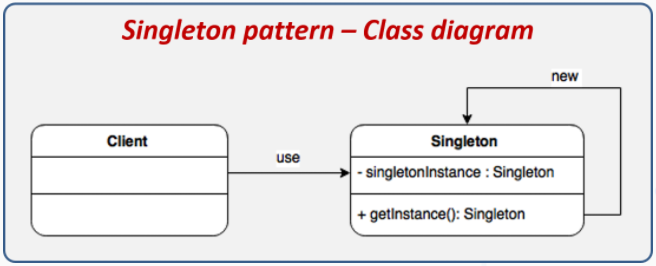
\includegraphics[width=5cm]{./img/imagen1.png} 
            \end{center}
		\item \textbf{Participantes :}	
        \begin{itemize}
            \item \textbf{	Client:}	
            \begin{itemize}
                Componente que desea obtener una instancia de la clase Singleton.
            \end{itemize}
        \item \textbf{Singleton:}	
            \begin{itemize}
                Clase que implementa el patrón Singleton, de la cual únicamente se podrá tener una instancia durante toda la vida de la aplicación[7].  	
            \end{itemize}
        \end{itemize}    

		\item \textbf{Aplicabilidad :}\\ Usar cuando: 
        \begin{itemize}
            \item Deba haber exactamente una instancia de una clase y ésta deba ser accesible a los clientes desde un punto de acceso conocido.  	
            \item La única instancia debería ser extensible mediante herencia y los clientes deberían ser capaces de utilizar una instancia extendida sin modificar su código[8]. 	
        \end{itemize}

		\item \textbf{Consecuencias:} 
        \begin{itemize}
            \item Acceso controlado a la única instancia. Puede tener un control estricto sobre cómo y cuando acceden los clientes a la instancia.   	
            \item Espacio de nombres reducido. El patrón Singleton es una mejora sobre las variables globales. 	   
            \item Permite el refinamiento de operaciones y la representación. Se puede crear una subclase de Singleton.   
            \item Permite un número variable de instancias. El patrón hace que sea fácil cambiar de opinión y permitir más de una instancia de la clase Singleton[8].  	
        \end{itemize}
	\end{itemize}
	
	
    \\
    \item \textbf{EJEMPLO DE IMPLEMENTACIÓN}
    \begin{center}
        \includegraphics[width=5cm]{./img/imagen4.png} 
    \end{center}

    \item \textbf{CODIGO}
    \begin{center}
        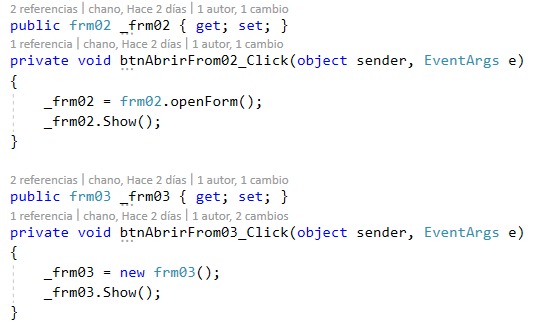
\includegraphics[width=5cm]{./img/Singleton1.png} 
    \end{center}
    \begin{center}
        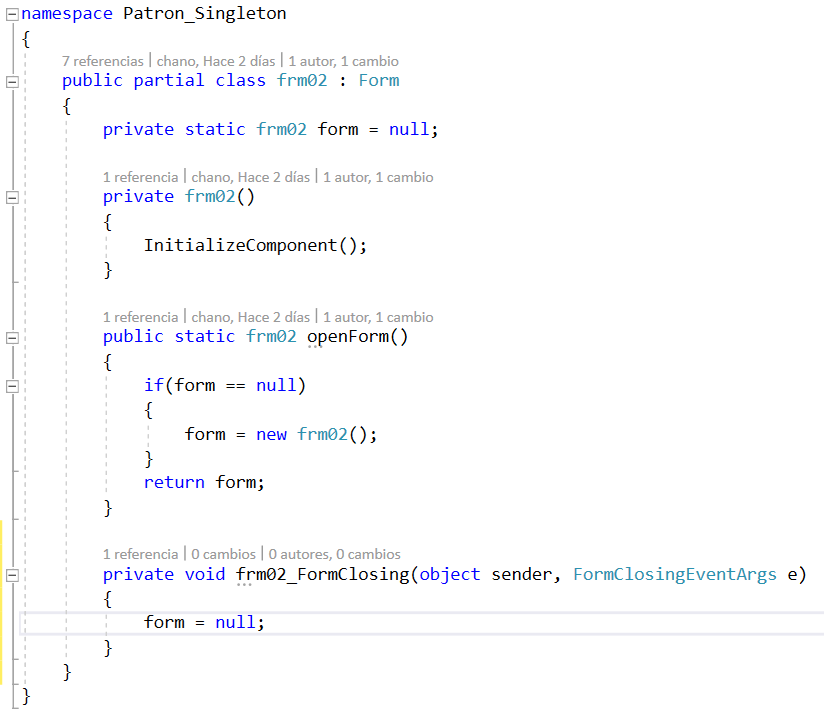
\includegraphics[width=5cm]{./img/Singleton2.png} 
    \end{center}
    \begin{center}
        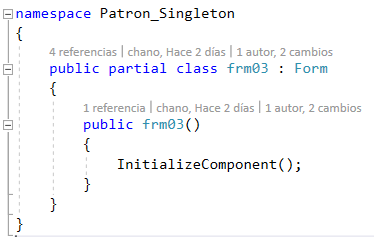
\includegraphics[width=5cm]{./img/Singleton3.png} 
    \end{center}
	
    \item \textbf{Patrones de diseño estructurales  }
	\\
	\\Los patrones estructurales nos ayudan a definir la forma en la que los objetos se componen[1]. Los patrones estructurales son:
	\begin{itemize}
		\item \textbf{Adapter:}	Permite a un cliente trabajar con clases cuya interfaz no posee una interfaz permitida en un sistema específico. Este patrón adapta la interfaz del objeto externo al de las clases del sistema al que se integra.  
		\item \textbf{Bridge:} Desacopla la abstracción de una clase de su implementación, permitiendo así, que varíen independientemente y se entregue flexibilidad y facilidad de mantenimiento al software.  
		\item \textbf{Composite:} Compone objetos relacionados en una jerarquía de tipo árbol. Este patrón de diseño le permite al cliente tratar de la misma manera un objeto y un grupo de objetos. 
		\item \textbf{Decorator:}	Añade responsabilidades adicionales a un objeto en tiempo de ejecución.  
		\item \textbf{Flyweight:}  Permite apoyarse en la copia de objetos complejos en un sistema que requiere la instanciación de un gran número de objetos con una estructura similar.  
		\item \textbf{Facade:} Provee una interfaz que representa las interfaces de los subsistemas del software. Además, facilita el uso de un sistema complejo con muchas relaciones directas al cliente.  
		\item \textbf{Proxy:} Restringe el acceso a un objeto para evitar su creación o participación precoz en el sistema. Usualmente, trata a objetos complejos o de gran tamaño. 
        \\
        \\
    \end{itemize}

    %%-------------------------------
    \item \textbf{PATRON DECORATOR} \\
    El patrón decorator está diseñado para solucionar problemas donde la jerarquía con subclasificación no puede ser aplicada, o se requiere de un gran impacto en todas las clases de la jerarquía con el fin de poder lograr el comportamiento esperado. Decorator permite al usuario añadir nuevas funcionalidades a un objeto existente sin alterar su estructura, mediante la adición de nuevas clases que envuelven a la anterior dándole funcionamiento extra[1]. 
	\begin{itemize}
		\item \textbf{OBJETIVO :}	\\Su función es determinar como las clases y objetos se combinan para formar estructuras.
        Estas estructuras permitirán que se agreguen nuevas funcionalidades.
        
        \begin{center}
            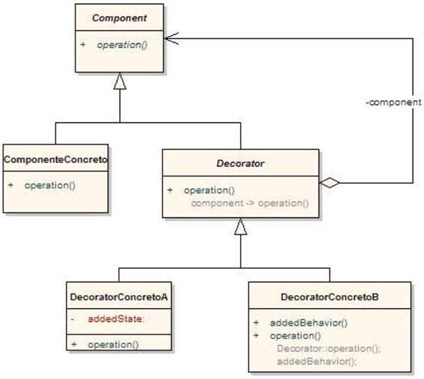
\includegraphics[width=5cm]{./img/Imagen5.png} 
        \end{center}
        \\

		\item \textbf{MOTIVACIÓN  :} \\Dotar de funcionalidades dinámicamente a objetos mediante composición. Es decir, vamos a decorar los objetos para darles más funcionalidad de la que tienen en un principio.
        Esto es algo verdaderamente útil cuándo queremos evitar jerarquías de clases complejas. La herencia es una herramienta poderosa, pero puede hacer que nuestro diseño sea mucho menos extensible.
        

		\item \textbf{APLICACIONES  :} \\
        El patrón se utiliza en los casos siguientes: 
            \begin{itemize}
                \item Añadir responsabilidades a objetos individuales de forma dinámica y transparente   	
                \item Responsabilidades de un objeto pueden ser retiradas	   
                \item Cuando la extensión mediante la herencia no es viable   
                \item Hay una necesidad de extender la funcionalidad de una clase, pero no hay razones para extenderlo a través de la herencia.  	
                \item Existe la necesidad de extender dinámicamente la funcionalidad de un objeto y quizás quitar la funcionalidad extendida.
            \end{itemize}
            \begin{center}
			    \includegraphics[width=5cm]{./img/imagen6.png} 
            \end{center}
            \begin{itemize}
                \item El Cliente realiza una operación sobre el DecoratorA.   	
                \item El DecoratorA realiza la misma operación sobre DecoradorB.   
                \item El decoradorB realiza una acción sobre ConcreteComponente. 
                \item El DecoradorB ejecuta una operación de decoración.  	
                \item El DecoradorA ejecuta una operación de decoración.	
                \item El Cliente recibe como resultado un objeto decorado por todos los Decoradores, los cuales encapsularon el Component en varias capas.
            \end{itemize}
		   
	\end{itemize}
	
	\item \textbf{DIAGRAMA DE ARQUITECTURA :}	\\
        Mediante la implementación del patrón de diseño Decorator crearemos una aplicación que nos permite procesar un mensaje en capas, donde cada capa se encargará de procesar un mensaje a diferente nivel.
        
        \begin{center}
            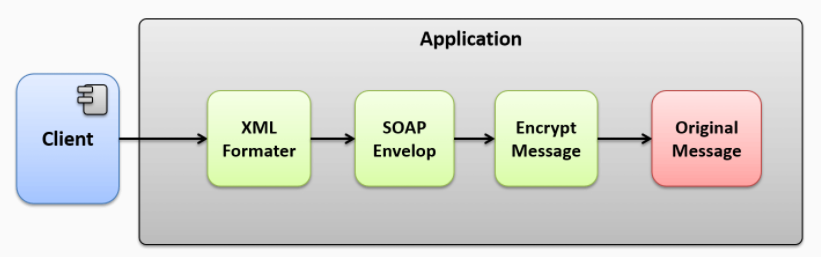
\includegraphics[width=5cm]{./img/Imagen7.png} 
        \end{center}
        \\

        \begin{itemize}
        \item \textbf{EJEMPLO DE IMPLEMENTACION:}	
        
        \begin{center}
            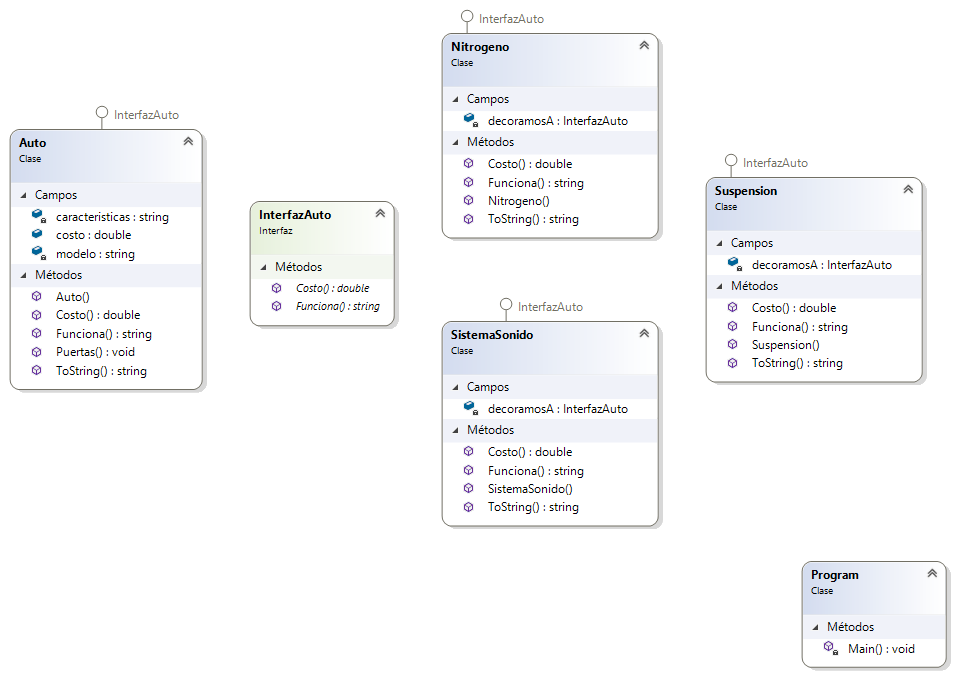
\includegraphics[width=5cm]{./img/Imagen8.png} 
        \end{center}
        \\

        \end{itemize} 

        
    \item \textbf{CODIGO}
    \begin{center}
        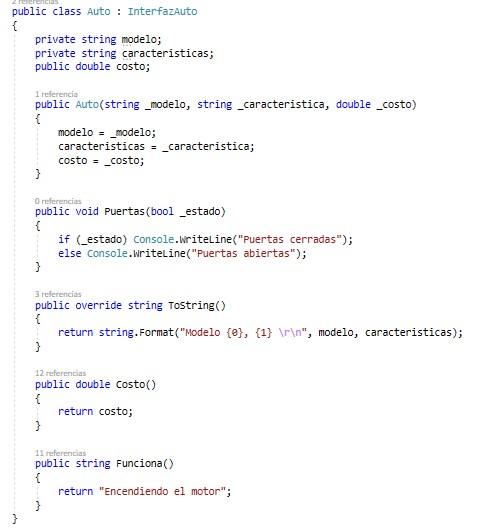
\includegraphics[width=5cm]{./img/Decorator1.jpg} 
    \end{center}
    \begin{center}
        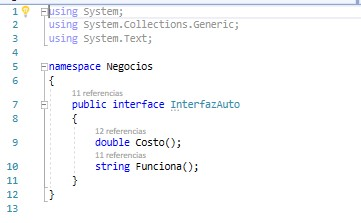
\includegraphics[width=5cm]{./img/Decorator2.jpg} 
    \end{center}
    \begin{center}
        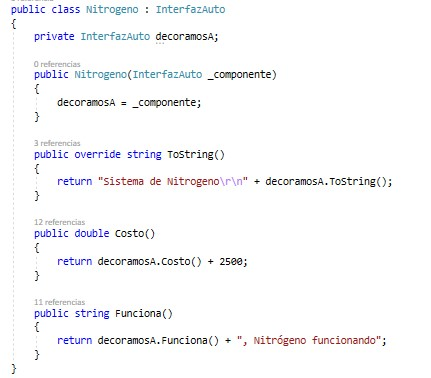
\includegraphics[width=5cm]{./img/Decorator3.jpg} 
    \end{center}

	
    \item \textbf{Patrones de Diseño de Comportamiento }
	\\
	\\Los patrones comportamentales nos ayudan a definir la forma en la que los objetos interactúan entre ellos[1]. Los patrones de comportamiento son:
    
	\begin{itemize}
		\item \textbf{Chain of responsibility:}	Evita el acoplamiento entre el objeto receptor y emisor de un mensaje específico. El patrón transfiere la responsabilidad a un objeto disponible.  
		\item \textbf{Command:} Encapsula una petición como un objeto para permitir su parametrización.   
		\item \textbf{Interpreter:} Permite definir una representación para su gramática y solucionar el mismo problema recurrente desde el contexto al que pertenece.  
		\item \textbf{Iterator:}	Proporciona una manera de acceder a un objeto agregado sin exponer su estructura interna.  
		\item \textbf{Mediator:}  Permite el bajo acople entre un conjunto de clases asignándole la implementación de los métodos a una sola clase.   
		\item \textbf{Memento:} Captura y externaliza el estado interno de un objeto para que éste pueda variar y volver al estado inicial en cualquier tiempo.   
		\item \textbf{State:} Permite a un objeto cambiar su comportamiento con base en los cambios de su estado interno.  
        \item \textbf{Strategy:} Permite encapsular algoritmos o funcionalidades específicas y hacerlas intercambiables. Este patrón de diseño le permite al algoritmo variar sin depender del cliente.  
        \item \textbf{Template Method:} Define el esqueleto de un algoritmo y permite cambiar ciertos pasos del mismo en las subclases. Estos cambios no afectan al algoritmo original.  
        \item \textbf{Visitor:} Permite adicionar funcionalidades a una clase existente sin afectar su estructura. 
        \item \textbf{Observer:} Define una dependencia de uno a muchos entre un conjunto de objetos para actualizarlos automáticamente una vez el objeto principal cambie su estado interno. 
        \\
        \\
    \end{itemize}


    %%-------------------------------
    \item \textbf{PATRON ITERATOR} \\
    Es un mecanismo de acceso a los elementos que constituyen una estructura de datos para la utilización de estos sin exponer su estructura interna. 
    El patrón Iterator proporciona un acceso secuencial a una colección de objetos a los clientes sin que éstos tengan que preocuparse de la implementación de esta colección. 
    
	\begin{itemize}
		\item \textbf{OBJETIVO :}	\\Proporcionar una forma de acceder a los elementos de una colección de objetos de manera secuencial sin revelar su representación interna. 
        Define una interfaz que declara métodos que permitan acceder secuencialmente a la colección[3].
         
        \begin{center}
            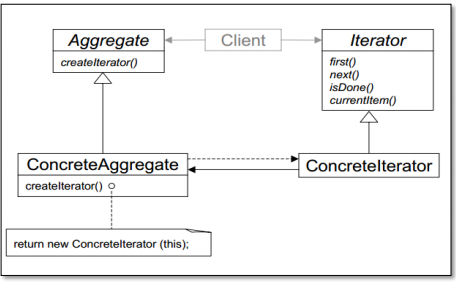
\includegraphics[width=5cm]{./img/Imagen9.png} 
        \end{center}
        \\
		\item \textbf{MOTIVACIÓN  :}\\ El patrón surge del deseo de acceder a los elementos de un contenedor de objetos (por ejemplo, una lista) sin exponer su representación interna. Además, es posible que se necesite más de una forma de recorrer la estructura siendo para ello necesario crear modificaciones en la clase. 
        La solución que propone el patrón es añadir métodos que permitan recorrer la estructura sin referenciar explícitamente su representación. La responsabilidad del recorrido se traslada a un objeto iterador.  
        El problema de introducir este objeto iterador reside en que los clientes necesitan conocer la estructura para crear el iterador apropiado
         

		\item \textbf{APLICACIONES  :}\\ El patrón se utiliza en los casos siguientes:  
            \begin{itemize}
            \item Es necesario realizar un recorrido de acceso al contenido de una colección sin acceder a la representación interna de esta colección. 
            \item Debe ser posible gestionar varios recorridos de forma simultánea.
            \end{itemize}   
        
            
		\item \textbf{CONSECUENCIAS  :}\\	Los iteradores simplifican la interfaz de las colecciones, ya que la interfaz de los recorridos se encuentra en los iteradores y no en la clase que corresponde a la estructura en cuestión. 
        Permite variaciones en el recorrido de una colección. 
        Para cambiar el algoritmo de recorrido basta cambiar la instancia de Iterator concreta  Nuevos recorridos mediante nuevas subclases de Iterator  
        Se puede tener más de un recorrido en progreso al mismo tiempo por cada colección
        
        
	\end{itemize}
	
	\item \textbf{DIAGRAMA DE CLASES :}	\\
    Los métodos más comunes son:

    \begin{itemize}
        \item \textbf{hasNext  :} Método que regresa un booleano para indicar si existen más elementos en la estructura por recorrer. True si existen más y false si hemos llegado al final y no hay más elementos por recorrer.
        \item \textbf{next  :} Regresa el siguiente elemento de la estructura de datos.
        \end{itemize} 

        \begin{center}
            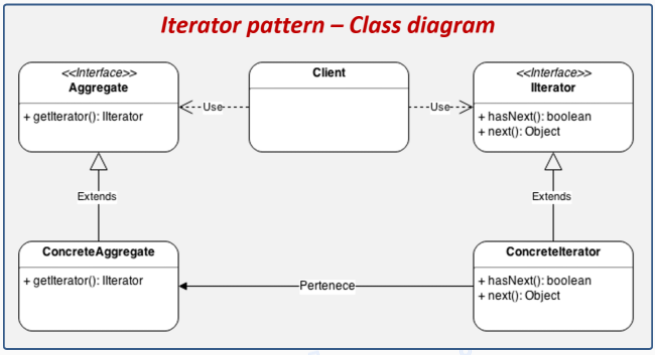
\includegraphics[width=5cm]{./img/Imagen10.png} 
        \end{center}
        \\
        Los elementos del patrón Iterator se describen a continuación:

        \begin{itemize}
            \item \textbf{Client  :} Actor que utiliza al Iterator.
            \item \textbf{Aggregate  :} Interface que define la estructura de las clases que pueden ser iteradas.
            \item \textbf{ConcreteAggregate  :} Clase que contiene la estructura de datos que deseamos iterar.
            \item \textbf{IIterator  :} Interface que define la estructura de los iteradores, la cual define los métodos necesarios para poder realizar la iteración sobre el ConcreteAggregator.
            \item \textbf{ConcreteIterator  :} Implementación de un iterador concreto, el cual hereda de IIterator para implementar de forma concreta cómo iterar un ConcreteAggregate.
            \end{itemize} 


        \begin{itemize}
        \item \textbf{DIAGRAMA DE ARQUITECTURA:}	\\
        Patrón de diseño Iterator crearemos una aplicación que nos permita recorrer una estructura organizacional jerárquica, mediante la implementación de un iterador, el cual nos permitirá recorrer todo el árbol de la estructura de forma secuencial.
        \begin{center}
            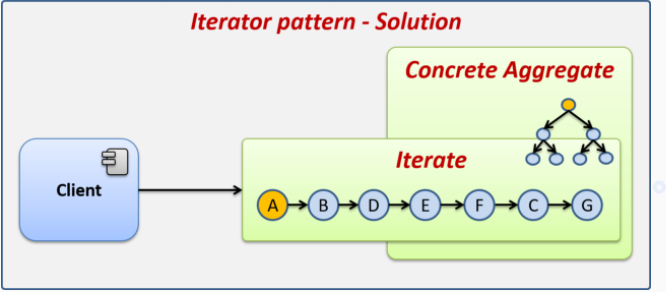
\includegraphics[width=5cm]{./img/Imagen11.png} 
        \end{center}
        \\

        \end{itemize} 

    \item \textbf{EJEMPLO DE IMPLEMENTACIÓN}
    \begin{center}
        \includegraphics[width=5cm]{./img/imagen12.png} 
    \end{center}
	
    \item \textbf{CODIGO}
    \begin{center}
        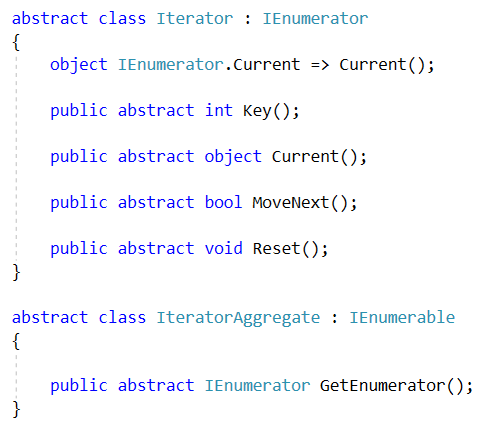
\includegraphics[width=5cm]{./img/Iterator1.png} 
    \end{center}
    \begin{center}
        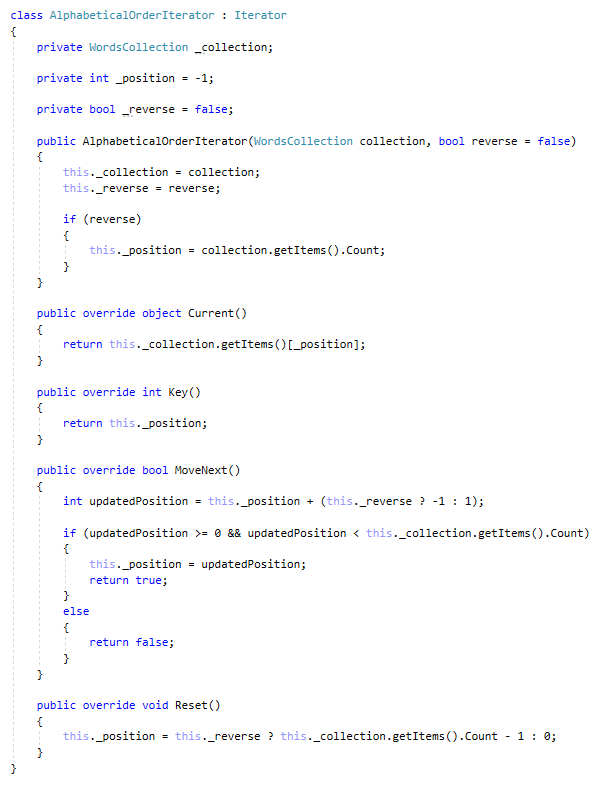
\includegraphics[width=5cm]{./img/Iterator2.png} 
    \end{center}
    \begin{center}
        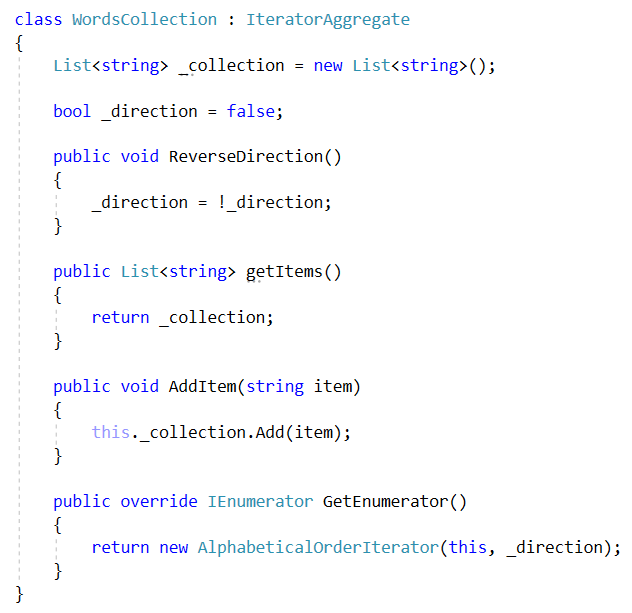
\includegraphics[width=5cm]{./img/Iterator3.png} 
    \end{center}
    \begin{center}
        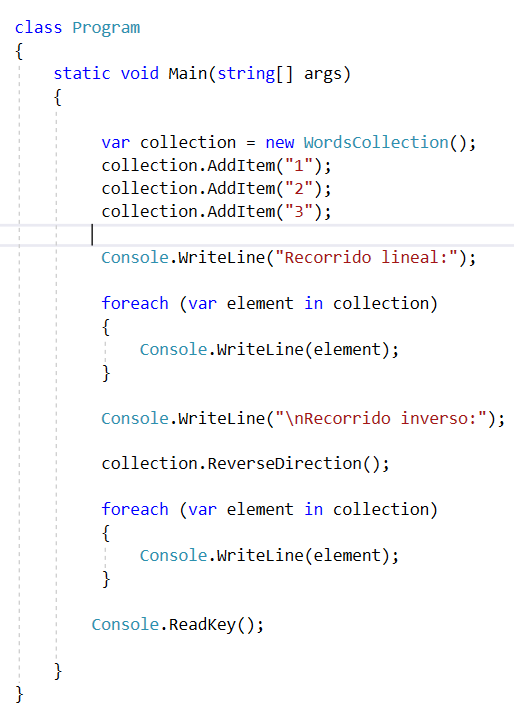
\includegraphics[width=5cm]{./img/Iterator4.png} 
    \end{center}
    \begin{center}
        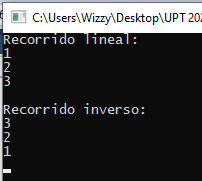
\includegraphics[width=5cm]{./img/Iterator5.png} 
    \end{center}
    %%-------------------------------
\section{Conclusiones}
\begin{itemize}
    En este artículo se ha pretendido introducir al lector en el mundo de los patrones software, pero partiendo desde la perspectiva inicial de este concepto.
    Se ha buscado familiarizar al lector con el concepto de patrón, con sus características y sus peculiaridades, más que con su utilización en el ámbito del Diseño Orientado a Objeto para construir aplicaciones software, con el fin de evitar caer en los falsos mitos y errores, causados por el desconocimiento y la falta de comprensión, propios de un acercamiento poco exhaustivo a una nueva área de conocimiento. 
    Se ha querido recoger en este artículo una amplia lista de referencias, a las que cualquier lector interesado pueda acceder para profundizar más en este interesante campo.
\end{itemize}


\section{Recomendaciones}
\begin{itemize}
	Al desarrollar aplicaciones robustas y fáciles de mantener, debemos cumplir ciertas “reglas”. Lo pongo entre comillas porque aunque estas reglas de diseño son recomendables (muy recomendables), no son obligatorias. Siempre podemos decidir no aplicarlas. Aunque si no lo hacemos, hay que ser conscientes de la razón de no aplicarlas y de sus consecuencias.
Los patrones de diseño nos ayudan a cumplir muchos de estos principios o reglas de diseño. Programación SOLID, control de cohesión y acoplamiento o reutilización de código son algunos de los beneficios que podemos conseguir al utilizar patrones.

\end{itemize}



%------------------------------------------------
%-----------------------------------------------------------------
\section{Bibliografía}\label{sec:6}
\begin{itemize}
\item [1] Erich Gamma, Richard Helm, Ralph Johnson, John Vlissides. (1994). Design Patterns: Elements of Reusable Object-Oriented Software. EEUU: Addison-Wesley.
\item [2] Coplien, James O. and Schmidt, Douglas (editors). “Pattern Languages of Program Design”. Addison-Wesley. 1995.
\item [3] Appleton, Brad. “Patterns and Software: Essential Concepts and Terminology”. http://www.enteract.com/~bradapp/docs\\/patterns-intro.html. November 1997.
\item [4] López Tallón, Alberto. “Patrones de Diseño. Reutilización de Ideas”. Revista Profesional para Programadores (RPP). Nº43: 54-58. Septiembre, 1998.
\item [5] Gamma, Erich, Helm, Richard, Johnson, Ralph and Vlissides, John. “Design Patterns. Elements of Reusable Object-Oriented Software”. Addison-Wesley, 1995.
\item [6] Alan Shalloway James R. Trott. (2004). Design Patterns Explained: A New Perspective on Object Oriented Design, 2nd Edition (Software Patterns). EEUU: Addison-Wesley.
\item [7] Source Making. (2015). Singleton Design Pattern. Recuperado de https://sourcemaking.com/design\_patter\\ns/singleton
\item [8] Tutorials Point. (2016). Design Pattern - Singleton Pattern. Recuperado de https://www.tutorialspoint.com/design\_\\pattern/singleton\_pattern.htm
\end{itemize}
% Bibliografia.
%-----------------------------------------------------------------

\bibliographystyle{plain}
\bibliography{bibliografia}
\end{document}
